%-----------------------------------------------------------------------------%
\chapter{\babSatu}
%-----------------------------------------------------------------------------%

This chapter explains the background of this research and the problem to be
solved by this research.

%-----------------------------------------------------------------------------%
\section{Research Background}
%-----------------------------------------------------------------------------%

When the web platform was in its early stages, every part of a web application
was programmed manually. At that time, developing a web application required
extensive knowledge of how the web works. Depending on the web application, the
programmers might need deep understanding of the Hypertext Transfer Protocol
(HTTP), the Hypertext Markup Language (HTML), and other things such as
databases. If the web application was not programmed correctly, it could lead
to a lot of errors and security holes in the web application.

Web frameworks aim to solve this problem by providing a standard way to build
web applications. Web frameworks help eliminate the overhead of implementing
common parts of web applications such as the HTTP layer, the user interface
layer, and the database layer. By using a web framework, programmers can build
web applications more quickly and safely by focusing more on the business logic
of the web application itself instead of the more intricate details.

Among the widely-used web frameworks is Django, a free and open-source web
framework written in Python.\footnote{\url{https://djangoproject.com}} Django
encourages rapid development and clean, pragmatic design \cite{django}. Django
was designed to help developers build their website quickly and securely with
scalability in mind.

One of the main features of Django is an object-relational mapping (ORM) tool
in the database layer \cite{django}. Django's ORM tool provides an
object-oriented abstraction of the database by mapping data models (represented
as Python classes) to tables in a relational database. The columns of a
database table are defined as attributes (called fields) inside the model
class. Using Django's ORM tool, programmers can interact with the database by
writing Python code instead of writing Structured Query Language (SQL)
statements. The abstraction provided by Django's ORM tool also helps
programmers avoid common mistakes that can lead to security issues such as SQL
injections.

Relational database systems can be used to manage structured data in the form
of tables with strict standards. The tables in a relational database can be
linked (related) based on data that is common to each table. Relating the
tables is possible because relational database systems enforce the data to be
consistent with a defined schema. This consistency is implemented according to
the Atomicity, Consistency, Isolation, and Durability (ACID) properties of
relational database transactions \cite{abramova_nosql}. These properties
guarantee that the data is valid despite any events of power failures, errors,
and other accidents.

Meanwhile, there has been an increase in the popularity of non-relational
databases, commonly known as NoSQL databases \cite{paul_nosql}. NoSQL
encourages the simplicity of database design, which makes the process of
scaling the database to multiple clusters of machines easier
\cite{leavitt_nosql}. Instead of tables, most NoSQL databases store data in the
form of key-value stores, document stores, or graphs \cite{strauch_nosql}.
NoSQL databases are also considered as more flexible due to its dynamic schema.
For example, some document-based NoSQL databases store data in JavaScript
Object Notation (JSON) format, which means that the schema is defined in the
data itself.

However, NoSQL databases also have their own downsides. Most NoSQL databases do
not fully support the ACID principles found in relational databases
\cite{cattell_nosql}. Instead of the ACID principles, they focus on the
Basically Available, Soft state, and Eventually consistent (BASE) principles
\cite{abramova_nosql}. The BASE principles state that the data should be
available most of the time (it can support partial failures), the data does not
have to be consistent at all times (soft state), but the data is guaranteed to
be consistent at some point (eventually). In addition, they also lack the
ability to perform joins across tables due to their horizontal data
distribution \cite{pokorny_nosql} and the use of denormalized data, which makes
it harder to deal with entity relations.

To compete with NoSQL databases, some relational database systems have come up
with their own ways to provide more flexibility for the data model. Some of
them provide the option to combine structured data with some form of
semi-structured data, most commonly in JSON format \cite{mariadb_json}. This
combination gives all the benefits of using a relational database, while still
allowing the simplicity and flexibility of semi-structured data.

From version 1.9 until version 3.0, Django had provided an implementation of
\code{JSONField}. However, it was exclusively available for PostgreSQL. This
\code{JSONField} allowed its users to store and query JSON data in a relational
database column using the \code{JSONB} data type found only on PostgreSQL at
the time. Django officially supports PostgreSQL, SQLite, MySQL, MariaDB, and
Oracle Database backends. Over the years since the initial PostgreSQL
\code{JSONField} implementation, those database systems have developed their
own support for dealing with JSON data. However, Django had yet to implement
\code{JSONField} for database backends other than PostgreSQL.

The limited support for \code{JSONField} prompted the Django community to
create their own \code{JSONField} implementations for other database backends.
Some of them target one specific database backend and utilize various functions
provided by the database system to add extended querying capabilities
\cite{mysql_jsonfield} \cite{oracle_jsonfield}. Some other implementations
focus on cross-database support, so they are only implemented as text-based
fields that do not have any extended querying capabilities
\cite{ryan_jsonfield}.

The individual efforts for implementing \code{JSONField} result in the
abundance of third-party \code{JSONField} packages on PyPI.\footnote{The Python
Package Index (PyPI) is a software repository for the Python programming
language.} Some of them are very popular, such as the \mbox{jsonfield} package
that has more than 1100 stars on GitHub \cite{ryan_jsonfield}. While this
indicates a popular demand for \code{JSONField}, it also indicates a
fragmentation problem as people use different \code{JSONField} packages. Thus,
there's a motivation to bring \code{JSONField} into Django's core model fields.

There's also a motivation to implement additional validations for JSON data in
a \code{JSONField}. By default, the validation for JSON data on the database
level only validates the syntax and not the information contained in the data
iself. Meanwhile, the flexibility of JSON data in a \code{JSONField} might
introduce invalid information or abnormalities within the data. For example,
the data might refer to a nonexisting record in one of the database tables. To
ensure the correctness of \code{JSONField} data, additional validations need to
be implemented.

In addition, recent studies showed interest in measuring the performance of
relational databases in handling JSON data. Relational databases are not
dedicated for storing JSON data, so they may not perform well compared to NoSQL
databases. However, recent benchmarks by EnterpriseDB showed that PostgreSQL
outperformed MongoDB in varied workloads with JSON data
\cite{enterprisedb_benchmark}.\footnote{MongoDB is one of the most popular
document-oriented NoSQL database systems.} Some extensive benchmarks on
PostgreSQL, MySQL, and MongoDB also showed that the performance differences
were not significant, especially for smaller documents \cite{dolgov_benchmark}.
However, these benchmarks were done directly on the database systems instead of
using an ORM tool. Therefore, further studies of relational databases'
performance in handling JSON data using an ORM tool would provide new insights
on this topic.

With the motivations described in the previous paragraphs, this research aimed
to implement \code{JSONField} in Django, demonstrate additional validations for
\code{JSONField}, and provide an analysis of \code{JSONField} performance. The
new implementation of \code{JSONField} would have cross-database support,
extended querying support, and compatibility with the previous \code{JSONField}
implementation. Additional validations for \code{JSONField} would be
demonstrated by creating a Django project that would utilize Django's
validation features. Finally, the JSON performance analysis would be done on
all database systems supported by Django, using Django's ORM tool in a Django
project. If these targets were achieved, they would hopefully benefit the
Django community by making \code{JSONField} available from within Django
itself, with additional validation examples, and performance insights for
consideration of using \code{JSONField}.

%-----------------------------------------------------------------------------%
\section{Research Questions}
%-----------------------------------------------------------------------------%

Based on the aforementioned research background, the following questions are
constructed for this research:

\begin{enumerate}
    \item How can \code{JSONField} in Django be reimplemented with
          cross-database support and compatibility with the previous
          \code{JSONField} implementation?
    \item How can Django users enforce validation rules on a \code{JSONField}?
    \item How is the performance of the cross-database \code{JSONField} on all
          of the database backends supported by Django?
\end{enumerate}

%-----------------------------------------------------------------------------%
\section{Research Objectives}
%-----------------------------------------------------------------------------%

The objectives of this research are to:

\begin{itemize}
    \item Implement a new \code{JSONField} that can be used on all database
          backends supported by Django.
    \item Demonstrate how semi-structured data in a \code{JSONField} can be
    validated.
    \item Provide a performance analysis of \code{JSONField} across different
          database backends.
\end{itemize}

%-----------------------------------------------------------------------------%
\section{Research Benefits}
%-----------------------------------------------------------------------------%

This research would hopefully bring the following benefits:

\begin{itemize}
    \item Provide Django users with a \code{JSONField} that has a consistent
          experience on all database backends supported by Django.
    \item Give insights to Django users about the inner workings, validation
          examples, and performance considerations of \code{JSONField}.
\end{itemize}

%-----------------------------------------------------------------------------%
\section{Research Scope}
%-----------------------------------------------------------------------------%

The following assumptions were made prior to the execution of this research:

\begin{itemize}
    \item The \code{JSONField} implementation would be submitted as a pull
          request and merged to the upstream Django repository instead of being
          made as a separate package.
    \item The primary focus of this research would be on implementing the model
          field type of \code{JSONField}, with the form field type as a
          secondary priority.
    \item The \code{JSONField} implementation has to take into account the
          limitations of each database backend, so there may be features that
          behave differently or are not supported on some database backends.
\end{itemize}

%-----------------------------------------------------------------------------%
\section{Research Position}
%-----------------------------------------------------------------------------%

\begin{figure}
	\centering
    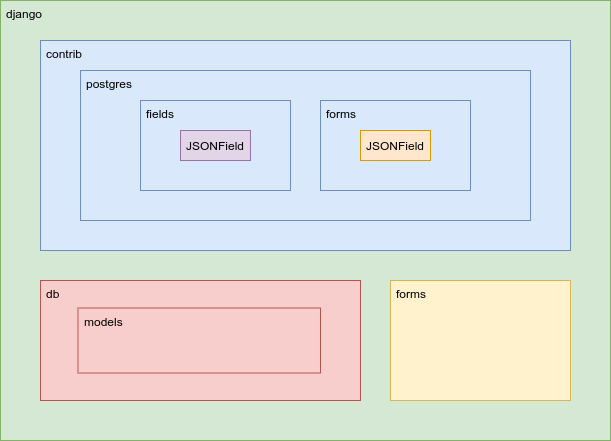
\includegraphics[width=0.85\textwidth]{pics/position1.png}
	\caption{\code{JSONField} classes in Django prior to this research.}
	\label{fig:position1}
\end{figure}

Before this research, the existing \code{JSONField} implementation was included
in the \code{django.contrib.postgres.fields} and
\code{django.contrib.postgres.forms} modules \cite{django30_modeljsonfield,
django30_formjsonfield}. The \code{django.contrib.postgres} module contains
model fields, form fields, and other features that only work with the
PostgreSQL database backend. The locations of the \code{JSONField} classes in
Django prior to this research are illustrated by \autoref{fig:position1} (note
that other Django modules are omitted for brevity).

\begin{figure}
	\centering
    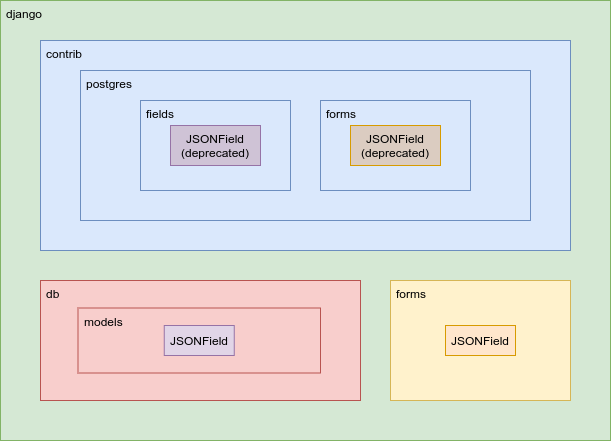
\includegraphics[width=0.85\textwidth]{pics/position2.png}
	\caption{\code{JSONField} classes in Django after this research.}
	\label{fig:position2}
\end{figure}

This research would bring \code{JSONField} and other related classes to the
\code{django.db.models} module for the model field and to the
\code{django.forms} module for the form field. Consequently, the previous
implementations would be deprecated as of the new Django release. The previous
implementations would also be removed in the next major release of Django.

\begin{figure}
	\centering
    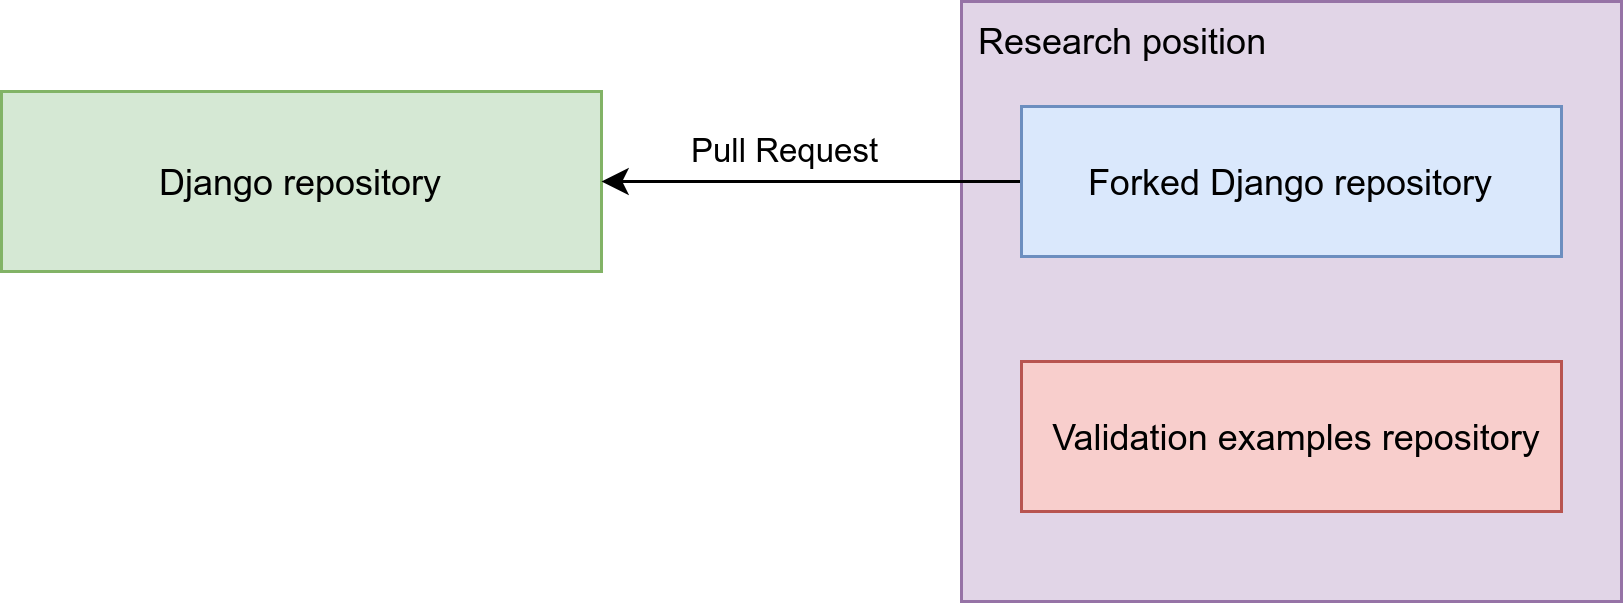
\includegraphics[width=0.85\textwidth]{pics/position3.png}
	\caption{The position of this research.}
	\label{fig:position3}
\end{figure}

This research is mainly split into two parts: the \code{JSONField}
implementation and the analysis demonstrations. The \code{JSONField}
implementation part of the research would be done on a Git branch in a GitHub
fork of the Django repository. The branch would be submitted as a pull request
to the Django repository to fix ticket \#12990 on the Django issue tracker
\cite{ticket_12990}. This would allow the Django contributors to review the
code and give feedback on the implementation. The data validation and
performance benchmarking analysis demonstrations would be done in a separate
repository in the form of two small Django projects. The position of this
research is illustrated by \autoref{fig:position3}.

\begin{figure}
	\centering
    
\includegraphics[width=0.25\textwidth]{pics/GSoC.png}
	\captionsource{The Google Summer of Code
        logo.}{\url{https://developers.google.com/open-source/gsoc/resources/marketing}}
	\label{fig:gsoc}
\end{figure}

The \code{JSONField} implementation would be done as part of the Google Summer
of Code 2019 program. Google Summer of Code (GSoC) is an annual program held by
Google that's focused on introducing students to open-source software
development. In GSoC, students work on a 3 month programming project under the
guidance of mentors from an open-source organization. The students are
compensated with a stipend from Google for their work. In turn, the
organizations can identify and bring in new contributors who implement new
features and hopefully continue to contribute to the organizations' projects.

%-----------------------------------------------------------------------------%
\section{Research Steps}
%-----------------------------------------------------------------------------%

The following steps were conducted for the research:

\begin{enumerate}
    \item Literature review \\
    This step focused on reading and understanding how the Django
    object-relational mapping (ORM) tool works, as well as JSON support on the
    database backends supported by Django. During this step, the underlying
    concepts of this research were studied in order to accomplish the research
    objectives.

    \item Experiments \\
    In this step, experiments were done by trying out existing \code{JSONField}
    implementations, which included the PostgreSQL implementation in Django, as
    well as third-party packages on the Python Package Index (PyPI). Some
    experiments were also done by modifying a third-party package to work
    better on different database backends.

    \item Implementation \\
    This step focused on the implementation of the \code{JSONField} model and
    form fields. This was initially done by copying the existing implementation
    from the \code{django.contrib.postgres} module to the
    \code{django.db.models} and \code{django.forms} modules. The tests for the
    existing implementation were also copied. From there, the work was to
    modify the \code{JSONField} implementation so that all tests could pass on
    all available database backends.

    After the \code{JSONField} implementation, this step was continued by
    implementing the data validation example and benchmarking. This included
    the creation of two small Django projects for demonstration purposes.

    \item Results Analysis \\
    In this step, the primary work was to document the different behaviors and
    support of the \code{JSONField} implementation on each database backend.
    This step also included analyzing the data validation and benchmarking
    implementations. For the benchmark, the analysis included comparing the
    performance of \code{JSONField} on all database backends.
\end{enumerate}

%-----------------------------------------------------------------------------%
\section{Report Structure}
%-----------------------------------------------------------------------------%

The structure of this report is as follows:

\begin{itemize}
    \item Chapter 1 \babSatu \\
        This chapter covers the background, problem definition, objectives,
        scope, position, and steps of this research.
    \item Chapter 2 \babDua \\
        This chapter covers the results of the literature review done prior to
        executing the research.
    \item Chapter 3 \babTiga \\
        This chapter covers the plan and problem analysis to prepare for the
        implementation.
    \item Chapter 4 \babEmpat \\
        This chapter covers the \code{JSONField}, the data validation example,
        and the benchmarking implementations.
    \item Chapter 5 \babLima \\
        This chapter covers the analysis of the implementation results. This
        also covers the comparison of the benchmarking results between the
        database backends.
    \item Chapter 6 \kesimpulan \\
        This chapter covers the conclusions of the research and some
        recommendations for further research.
\end{itemize}
